\documentclass{amsart}

\usepackage[foot]{amsaddr}
\usepackage{amsmath}
\usepackage{amssymb}
\usepackage{amsthm}

\usepackage{braket}  % provides \set{ | }

\usepackage{graphicx}
\usepackage{subcaption}
\usepackage{booktabs}

\usepackage{hyperref}
\usepackage{xcolor}
\hypersetup{
    colorlinks,
    linkcolor={red!50!black},
    citecolor={blue!50!black},
    urlcolor={blue!80!black}
}

\theoremstyle{plain}
\newtheorem{theorem}{Theorem}[section]
\newtheorem{lemma}[theorem]{Lemma}
\newtheorem{proposition}[theorem]{Proposition}

\theoremstyle{definition}
\newtheorem{definition}[theorem]{Definition}
\newtheorem{example}[theorem]{Example}

\theoremstyle{remark}
\newtheorem{remark}[theorem]{Remark}

\begin{document}
	\title{Difference multisets}

	\author{Juris Evertovskis}
	\email{juris.evertovskis@lu.lv}

	\author{Juris Smotrovs}
	\email{juris.smotrovs@lu.lv}
	
	\address{Faculty of Computing, University of Latvia}

	\begin{abstract}
		Difference multiset is a combinatorial design---a multiset $M$ over a 
		group $G$ such that the differences of elements of $M$ produce every 
		element of $G$ in the same number of times. In this paper we obtain 
		multiple new constructions of difference multisets as well as some 
		constraints on structure of difference multisets. We paid special 
		attention to a few cases with small parameter values and managed to 
		find all of the difference multisets over some smaller algebraic 
		structures, e.g.\ $\mathbb Z_3, \mathbb Z_2^2$ and $\mathbb Z_2^3$. 
		It turned out that there is a link between difference multisets over 
		$\mathbb Z_3$ and Löschian numbers.

		\smallskip
		\noindent \textbf{\keywordsname.} Difference multisets, Difference covers, Löschian numbers
	\end{abstract}

	\maketitle
    
    \section{Introduction}
    \subsection{Difference multisets}

    Difference multiset is a combinatorial design similar to difference set. %But a multiset. 

    The classical difference set $D$ in a finite group $G$ is such a subset of $G$ that produces every non-zero $\gamma \in G$ the same number of times when taking the differences between elements of $D$. A simple example is $\set{0,1} \subset \mathbb Z_3$ as $1-0=1$ and $0-1=2$ thus producing both of the non-zero elements of $\mathbb Z_3$. 
%Curiosly, the same pair is also a difference set in $\mathbb Z_2$, but that's boring as $G$ is always a difference set of $G$. 
A less trivial and more famous example is the set $\set{1,2,4} \subset \mathbb Z_7$.

    If we take a multiset instead, we can produce the whole $G$, including the identity element. For example, considering the differences between elements of $\set{0,0,1} \subset \mathbb Z_3$ we obtain $\set{0,0,1,1,2,2}$. This is what is called a difference multiset. Note that we take differences between pairs of elements not an element and itself (i.e. there was $0-0=0$ as first zero subtracted from the second zero and vice versa but not the first zero from itself and no $1-1$).

    While difference sets have been studied at least since 1939 \cite{bose1939construction}, difference multisets were first investigated on their own in 1999 by Buratti \cite{buratti1999old} who noticed that such designs (and the related strong difference families) are indirectly used by other authors in constructions of various combinatorial designs. The paper defined the concept of a difference multiset and presented its basic properties and some constructions. The topic was developed further by other authors \cite{arasu2005cyclic, arasu2005regular} (they used the term ``regular difference covers'' instead of ``difference multisets'') who introduced new constructions and several nonexistence theorems.

    The results in the foundational articles are mostly analogous to those of difference sets, almost all of the constructions are based on some difference set construction. As a result the number of difference multisets constructed in a given finite group is proportional to that of difference sets which is unlikely to reflect the real situation as there are infinitely more multisets over a given finite $G$ than there are subsets. Some constructions producing difference multisets of arbitrary size over fixed $G$ were presented in \cite{momihara2009strong} and we strive to expand in this direction---constructing arbitrarily large multisets in fixed, mainly small algebraic structures.

\subsection{Synopsis}

    We study the difference multisets using a system of quadratic and linear equations on the multiplicities of their elements. We show that these multiplicities of any difference multiset over a loop are in a sense close to their average. This leads to the next idea of studying their digressions from the average which allows describing difference multisets with a simpler equation system.

    Using these tools we find a construction that allows to produce an infinite number of difference multisets over any quasigroup. Focusing on groups $\mathbb Z_2^i$, we obtain a more general construction that includes the previous one as a special case, and also provides all multisets for $\mathbb Z_2^i$ for at least $i \leq 3$.

    We also solve the problem of difference multisets of quasigroups of cardinality 3. Interestingly, the possible sizes of difference multisets over $\mathbb Z_3$ turn out to be Löschian numbers.
    

     
	\section{Definitions, notation and statement of the problem}
    When describing large or arbitrary multisets over a fixed group, it's convenient to use the multiplicity function $n$: the number of instances an element $\mu$ is found in a multiset $M$ will be denoted as $n(\mu,M)$ or simply $n_\mu$ if the multiset is obvious from the context.

Let $G$ be a commutative group and $M=\set{\mu_1, \mu_2, \ldots, \mu_k}$ be a multiset over $G$. Let us denote by $\mathcal D(M)$ the multiset generated by the differences of elements of $M$ with different indices: 
$\mathcal D (M) = \set{\mu_i-\mu_j \mid i, j \in \{1,2,\ldots,k\} \land i \neq j}$.

\begin{definition}
    \label{dms:def:dc}
    A multiset $M$ of cardinality $k$ is called a $(G,k)$-difference cover iff $\forall \gamma \in G \colon \gamma \in \mathcal D(M)$.
\end{definition}

In particular we are interested in difference covers 
for which $\mathcal D(M)$ is regular: it contains each element of $G$ the same number of times.

\begin{definition}
    \label{dms:def:dms}
    A $(G,k)$-difference cover $M$ is called a $(G,k)$-difference multiset (a.k.a.\ regular difference cover) if $\exists \lambda  \forall \gamma \in G \colon \lambda = n(\gamma, \mathcal D(M))$.
\end{definition}

The use of symbols $\lambda$ and $k$ is consistent with their roles as parameters of the common difference sets. They serve the same purpose here and we will also use the classic notation $v = |G|$. Commonly a $(G,k)$-difference multiset would be called a $(G,k,\lambda)$ (or $(v,k,\lambda)$) difference multiset, but we omit $\lambda$ as it is a function of $v$ and $k$ 
(see identity \eqref{apparatus:eq:parameters} below).


\subsection{The mathematical apparatus}
    \label{sec:apparatus}
    First, note that the cardinality of $(G,k)$-difference multiset is equal to the total of multiplicities. We will omit the summation index and bounds where they are clear from the context. Suppose that all sums are over $\mu \in G$ unless stated otherwise.
    \begin{equation}
        \label{apparatus:eq:ni}
        \sum {n_\mu} = k.
    \end{equation}
    
    Now let us restate definition \ref{dms:def:dms} in terms of $n$. Each element $\gamma$ must appear $\lambda$ times as a difference $(\gamma+\mu)-\mu$. For non-identity $\gamma$ we obtain the number of $\gamma$'s occurrences by multiplying the multiplicities $n_{\gamma+\mu} n_\mu$ and summing over $\mu \in Q$. For the identity we will use Kronecker delta to omit the trivial differences (i.e.\ $\mu_i-\mu_i$ where $M=\{\mu_1,\ldots,\mu_k\}$ is the multiset):
    \begin{equation}
        \label{apparatus:eq:system}
        \forall \gamma \in G \colon \sum (n_\mu(n_{\gamma+\mu}-\delta_{\gamma0})) = \lambda.
    \end{equation}
    
    We can observe that the number of non-trivial differences is equal to the number of $(G,k)$-difference multiset element pairs (sub-multisets of order $2$) $k(k-1)$ and it's required to contain each of the $v=|G|$ elements $\lambda$ times \cite{buratti1999old}:
    \begin{equation}
        \label{apparatus:eq:parameters}
        v\lambda = k(k-1).
    \end{equation}
(As is well known, a similar identity holds for the common difference sets.)
    
    These equations serve as the main tools in our investigation. Finding a $(G,k)$-difference multiset is the same as finding a set of non-negative integer $n_\mu$'s that satisfy the above equations. 
    
    It is useful to notice that equation \eqref{apparatus:eq:ni} defines a hyperplane and equations \eqref{apparatus:eq:system} define second-order surfaces. Under this interpretation we are looking for lattice points on the intersection of all the surfaces defined by these equations.

\subsection{Digressions}
\label{sec:digressions}
    By applying the substitution $n_\mu=\frac{k+d_\mu \sqrt k}v$ we can rewrite the previous equations in terms of digressions $d_\mu$:
    
    \begin{equation}
        \label{apparatus:eq:di}
        \sum {d_\mu} = 0
    \end{equation}
    
    \begin{equation}
        \label{apparatus:eq:dsystem}
        \forall \gamma \in G \colon \sum d_\mu d_{\gamma+\mu} = v (v \delta_{\gamma0}-1).
    \end{equation}
    
    This makes it a bit simpler to find a solution in terms of $d_\mu$, but the cost is that we must afterwards test if the solution produces integer $n_\mu$.
    

	
    \section{Main results}
    \subsection{Limits for multiplicities}
Considering difference multisets over an arbitrary abelian group 
one can notice that some of the surfaces defined by our equations 
are always the same. There is always the hyperplane 
$\sum {n_\mu} = k$ and the hypersphere $\sum n_\mu^2 = k + \lambda$ 
centered at the origin (see Figure \ref{general:figure:surfaces}). 

The second equation confines every multiplicity: 
$n_\mu \leq \sqrt{k+\lambda}$. By investigating the intersection
more thoroughly we discover that the multiplicities are actually 
bound to be near to their average $k/v$ (see Figure \ref{general:figure:limits}).

\begin{figure}
	\centering
	\begin{subfigure}[b]{0.5\textwidth}
		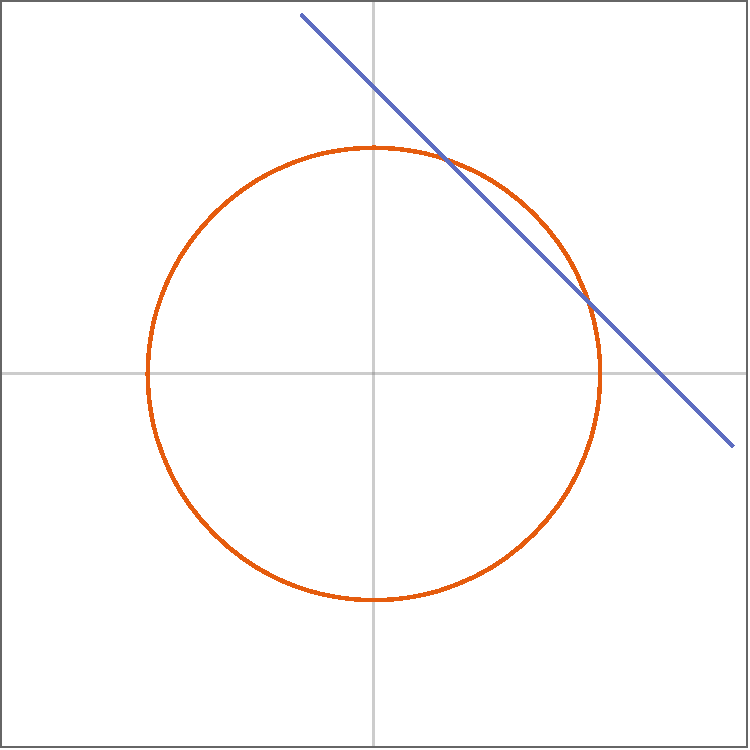
\includegraphics[width=\textwidth]{assets/surfacesIn2D}
	\end{subfigure}%
	~
	\begin{subfigure}[b]{0.5\textwidth}
		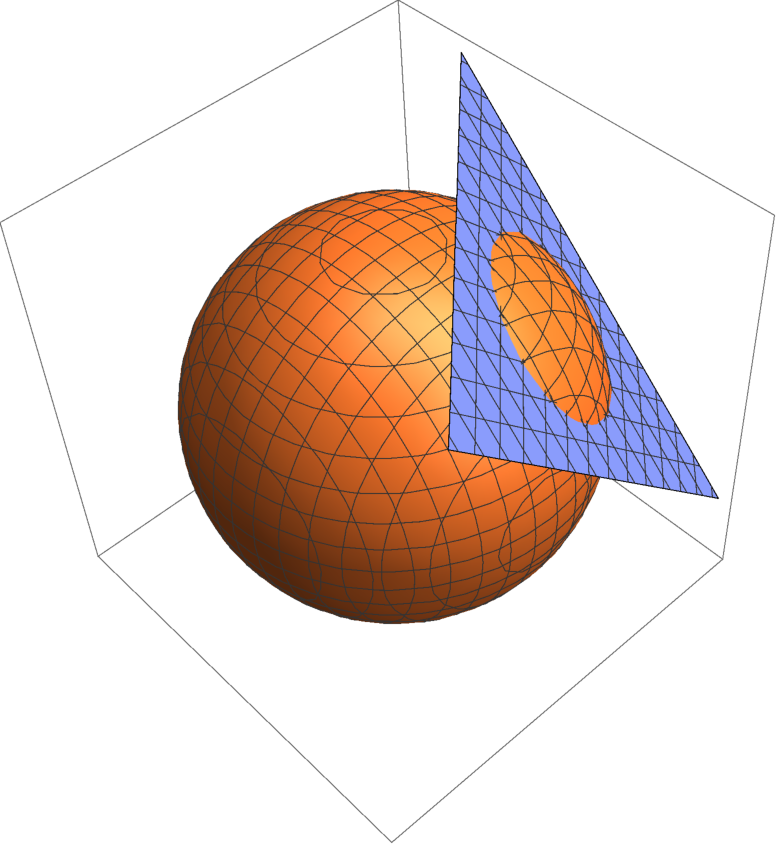
\includegraphics[width=\textwidth]{assets/surfacesIn3D}
	\end{subfigure}
	\caption{The $\sum {n_\mu} = k$ and $\sum n_\mu^2 = k + \lambda$ surfaces in two and three dimensions.}
	\label{general:figure:surfaces}
\end{figure}
	
\begin{theorem}
	\label{general:theorem:limits}
	If $M$ is a $(G,k)$-difference multiset and $|G|=v$ then
	\begin{equation}
		\forall \gamma \in G \colon\qquad \frac{k-(v-1)\sqrt k}{v} \leq n(\gamma,M) \leq \frac{k+(v-1)\sqrt k}{v}
	\end{equation}
\end{theorem}

\begin{proof}
	Take equation \eqref{apparatus:eq:system} for the identity element and equation \eqref{apparatus:eq:ni} as constraints:
	
	\begin{equation}
		\begin{cases}
			\sum {n_\mu} = k \\
			\sum (n_\mu(n_\mu-1)) = \lambda.
		\end{cases}
	\end{equation}
	
	Let us optimize $n_\gamma=n(\gamma,M)$ respecting the constraints. Add the first equation to the second and move all the terms to the left hand side:
	
	\begin{equation}
		\begin{cases}
			k - \sum {n_\mu} = 0 \\
			k + \lambda - \sum n_\mu^2 = 0.
		\end{cases}
	\end{equation}
	
	We apply the method of Lagrange multipliers to obtain the maximum and minimum of $n_\gamma$. 
	
	We use the following Lagrange function ($\lambda_1$ and $\lambda_2$ here is the standard Lagrange multiplier notation and have nothing in common with the parameter $\lambda$).
	
	\begin{equation}
		\mathcal L = n_\gamma - \lambda_1 (k - \sum n_\mu) - \lambda_2 (k + \lambda - \sum n_\mu^2)
	\end{equation}
	
	By a standard application of this method the bounds of the theorem statement are obtained. We omit the routine calculations.
\end{proof}

Theorem \ref{general:theorem:limits} suggests using digressions 
instead of multiplicities (thus simplifying the equations) and 
greatly reduces the amount of options for every $n_\gamma$. This 
simplification allows decent computer searches which enabled us to 
discover some of the patterns that led to results presented in this 
paper.
	
\begin{figure}
	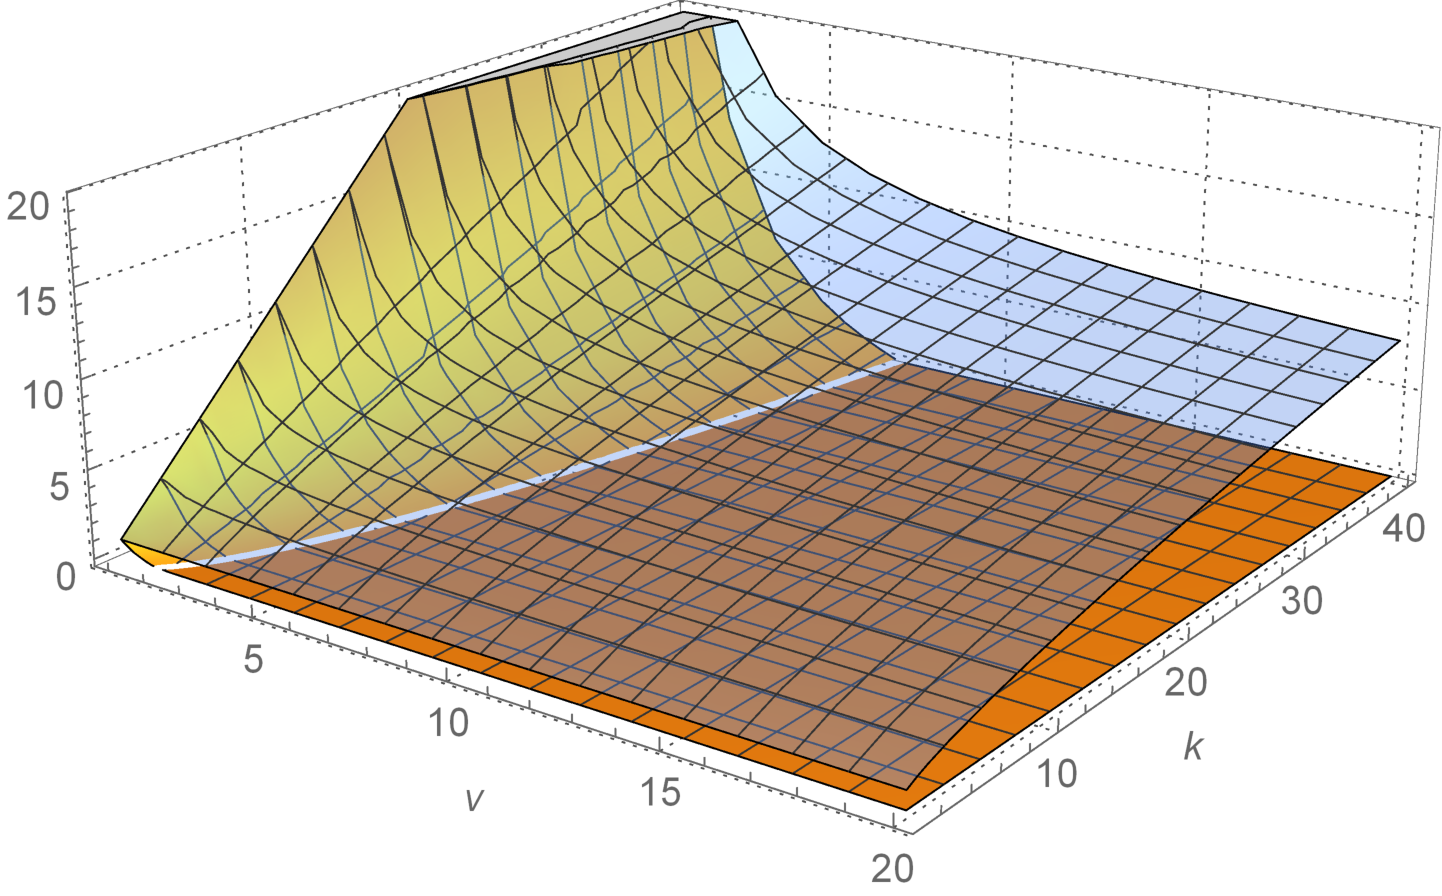
\includegraphics[width=\textwidth]{assets/boundingSurfaces}
	\caption{Lower and upper bounds for the values of $n_\gamma$ with respect to $v$ and $k$.}
	\label{general:figure:limits}
\end{figure}


\subsection{A family of difference multisets for every abelian group}
\label{sec:uni}
\begin{theorem}
	\label{regular:theorem:regular}
	If $\sqrt k$ is integer and congruent to $0$ or $\pm 1 \mod v$ then a $(G,k)$-difference multiset exists with the following digressions.
		\begin{itemize}
			\item If $\sqrt k \equiv 1 \mod v$ then $d_\mu = v-1$ for any single element $\mu$ and $d_{\nu \neq \mu} = -1$ for the other elements.
			\item If $\sqrt k \equiv -1 \mod v$ then $d_\mu =1-v$ for any single element $\mu$ and $d_{\nu \neq \mu} = 1$ for the other elements.
			\item Both of the above constructions if $\sqrt k \equiv 0 \mod v$.
		\end{itemize}
\end{theorem}

\begin{proof}
	The conditions on the values of $k$ and $d_\mu$ guarantee that the multiplicities $n_\mu=\frac{k+d_\mu \sqrt k}v$ are integers. It is left to demonstrate that they form a difference multiset.
	
	Considering equation \eqref{apparatus:eq:dsystem} for non-identity elements we can notice that the digression $\pm(v-1)$ (as any other digression) is involved in two of the products---once as $d_\mu$ and once as $d_{\gamma+\mu}$.

	Other $v-2$ products are $(\pm1)\cdot(\pm1)$, thus the condition is satisfied:
	
	\begin{equation}
		\sum d_\mu d_{\gamma+\mu} = 2(\pm(v-1)\cdot(\mp 1)) + (v-2)(\mp1)^2 = -v.
	\end{equation}

	The condition for the identity $\gamma=0$ is also satisfied:
	
	\begin{equation}
		\sum d_\mu^2  = \left( \pm (v-1) \right)^2 + (v-1) \left( \mp 1 \right)^2 = v^2 - v.
	\end{equation}

	It is straightforward to check that equation \eqref{apparatus:eq:di} is satisfied as well.
\end{proof}


\subsection{Difference multisets for cyclic groups}
Let us consider \eqref{apparatus:eq:dsystem} in matrix form 
\begin{equation}
\label{general:eq:matrix_eq}
	D d = \bf v
\end{equation}
where $d = (d_0, d_1, \ldots, d_{v-1})^T$, $\bf{v} = (v^2-v, -v, -v, \ldots)^T$ and $D_{\mu\nu} = d_{\mu+\nu}$, i.e.\ it is the Cayley table of the group in question.

For cyclic groups the matrix $D$ takes the form of an \emph{anticirculant} or \emph{left circulant} matrix:

\begin{equation}
	\label{general:eq:anticirculant_matrix}
	D =
	\begin{pmatrix}
		d_0 & d_1 & d_2 & \cdots & d_{v-1} \\ 
		d_1 & d_2 & d_3 & \cdots & d_0 \\
		d_2 & d_3 & d_4 & \cdots & d_1 \\
		\vdots & \vdots & \vdots & \ddots & \vdots \\
		d_{v-2} & d_{v-1} & d_0 & \cdots & d_{v-3} \\
		d_{v-1} & d_0 & d_1 & \cdots & d_{v-2} \\
	\end{pmatrix}.
\end{equation}

We will use the discrete Fourier transform:
\begin{equation}
	\mathcal F (y)_m = \sum_{j=0}^{v-1} y_j \omega^{-jm}
\end{equation}
where $\omega = \exp(\frac{2\pi \imath}v)$. Let us consider an equation $Ax=b$ with anticirculant matrix $A$. Applying the discrete Fourier transform to $b$ we obtain

\begin{equation}
	\label{general:eq:fourier_image}
	\mathcal F (b)_m = \mathcal F (a)_m \mathcal F ^*(x^*)_m,
\end{equation}
where $a$ is the first row of $A$.

This is particulary useful for equation \eqref{general:eq:matrix_eq} as the vector $d$ is also the first row of matrix $D$. The image of $\bf v=Dd$ is

\begin{equation}
	\mathcal{F} ({\bf v})_m = \mathcal{F}(d)_m \mathcal{F^*}(d^*)_m.
\end{equation}

As we are only interested in real $d$, we can simplify it further:

\begin{equation}
	\label{general:eq:dfourier}
	\mathcal{F} ({\bf v})_m = \mathcal{F}(d)_m \mathcal{F^*}(d)_m = |\mathcal{F}(d)_m|^2.
\end{equation}

Since ${\bf v} = (v^2-v, -v, -v, \ldots)^T$ we can find that $\mathcal{F}({\bf v}) = (0,v^2,v^2,\ldots)$ and \eqref{general:eq:dfourier} becomes
\begin{equation}
	\label{gen:eq:dfourierfinal}
	\left| \sum_{\mu=0}^{v-1} d_\mu \omega^{-\mu m} \right| = v (1-\delta_{m0}).
\end{equation}

\begin{theorem}
	\label{general:theorem:split_cycles}
	The digressions of a $(\mathbb Z_v, k)$-difference multiset are related via equation
	\begin{equation}
		\label{general:eq:split_cycles}
		\left| 
			\sum_{\kappa=0}^{v/m-1} \omega^{-m\kappa} \cdot 
			\sum_{\nu=0}^{m-1}  d_{\kappa+\nu v/m} 
		\right| = v
	\end{equation}
	where $m$ is any divisor of $v$ and $\omega = \exp(\frac{2\pi \imath}v)$.
\end{theorem}

\begin{proof}
	The theorem statement is obtained from \eqref{gen:eq:dfourierfinal}.
	
	Select a divisor $m$ of $v$. Then $\delta_{m0}=0$ on the right hand side. The left hand side is transformed and grouped into smaller cycles using the following relation:
	\begin{equation}
		\omega^{-m (\kappa+\nu v/m)}
		= \omega^{-m \kappa} \omega^{-\nu v}
		= \omega^{-m \kappa}.
	\end{equation}
\end{proof}

\begin{proposition}
	\label{general:theorem:even_cyclic}
	In difference multistes over cyclic groups of even cardinality $\sum_{\mu=0}^{v/2-1} d_{2\mu} = \pm \frac v2$ and $\sum_{\mu=0}^{v/2-1} d_{2\mu+1} = \mp \frac v2$.
\end{proposition}
\begin{proof}
	Take \eqref{general:eq:split_cycles} for $m=v/2$
	\begin{equation}
		\left| 
			\sum_{\mu=0}^{v/2-1} d_{2\mu} 
			- \sum_{\mu=0}^{v/2-1} d_{2\mu+1} 
		\right| = v.
	\end{equation}
	
	I.e.\ the total of even $d_\mu$'s and the total of odd $d_\mu$'s differ by $v$. Take into account that the grand total is $\sum d_\mu = 0$ and the proposition follows.
\end{proof}

\begin{remark}
	Similar relation also holds true for some other structures that are 
	not cyclic groups. For example in $\mathbb Z_2 \times \mathbb Z_2$
	with elements $\set{\mu, \nu, \zeta, \eta}$ in any order we have 
	$(d_\mu+d_\nu)-(d_\zeta+d_\eta)=\pm 4$.
\end{remark}


\subsection{Difference multisets over $\mathbb Z_2^m$}
\label{sec:z2i}
Consider $\mathbb Z_2^m$ as an affine space over $\mathbb Z_2$. For a chosen affine frame $F$, each element $\mu\in\mathbb Z_2^m$ can be represented by its affine coordinates: $\mu=(\mu_1, \mu_2, \ldots, \mu_m)$. For $i\in\{1,2,\ldots,m\}$ we define subspaces $H_i^F$ and $\widetilde H_i^F$ as follows:

\begin{equation}
    \mu \in H_i^F \iff 
        \begin{cases}
            \mu_j = 1 & \text{for } j < i \\
            \mu_i = 0
        \end{cases}
\end{equation}

\begin{equation}
    \mu \in \widetilde H_i^F \iff 
        \mu_j = 1 \text{ for } j \leq i
\end{equation}
and denote $\xi_i = \sum\limits_{j=0}^i (-2)^j=(1-(-2)^{i+1})/3$.

\begin{theorem}
    \label{z2i:theorem:construction}
    For an arbitrary affine frame $F$ of $\mathbb Z_2^m$ and integer $r \colon 0 < r < m$, the following construction produces a $(\mathbb Z_2^m, k)$-difference multiset iff $k$ is square and $v | \sqrt k$:
    \begin{enumerate}
        \item For each $\mu \in H_i^F$ where $i \leq r$, set $d_\mu = \xi_i$.
        \item Select element $\nu \in \widetilde H_r^F$.
        \item Set $d_\nu = (-1)^r v + \xi_{r+1}$.
        \item Set $d_\mu = \xi_{r+1}$ for all $\mu \in \widetilde H_r^F\setminus\{\nu\}$.
    \end{enumerate}
    A difference multiset is also obtained if the opposite sign is used on every $d_\mu$.
\end{theorem}

\begin{proof}
	For a selected $r \colon 0 < r < m$ this construction provides us with $2^{m-i}$ digressions of value $d_\mu=\xi_i$ for each $i$ ($1 \leq i\leq r$), $2^{m-r}-1$ digressions equal to $\xi_{r+1}$ and one digression equal to $(-1)^r 2^m+\xi_{r+1}$.
    
    It is easy to check that the equations $\sum d_\mu = 0$ and $\sum d_\mu^2 = v(v-1)$ are satisfied with these values.
    
    It remains to check the equations \eqref{apparatus:eq:dsystem} for non-identity $\gamma$.
    
    For $\gamma = (\gamma_1, \gamma_2, \ldots, \gamma_m)$ let $s$ be the smallest index for which $\gamma_s=1$. Then we can observe the following behaviour of $\gamma + \mu$:
    \begin{itemize}
        \item If $s > r$ then $\mu \in H_i^F \iff  \gamma + \mu \in H_i^F$ and $\mu \in \widetilde H_r^F \iff  \gamma + \mu \in \widetilde H_r^F$.
        \item If $s \leq r \land i < s$ for then $\mu \in H_i^F \iff  \gamma + \mu \in H_i^F$.
        \item If $s \leq r \land i = s$ then $\mu \in H_i^F \iff  \gamma + \mu \in \widetilde H_i^F$.
        \item If $s \leq r \land i > s \land i \leq r$ then $\mu \in H_i^F \iff  \gamma + \mu \in H_s^F$.
        \item If $s \leq r$ then $\mu \in \widetilde H_r^F \iff \gamma + \mu \in H_s^F$
    \end{itemize}
    
    We shall consider the case $s\leq r$ first. The value of \eqref{apparatus:eq:dsystem} is evaluated as follows
    
    \begin{equation}
        \begin{split}
            \sum d_\mu d_{\gamma+\mu}
              = & \sum\limits_{i<s} \sum\limits_{\mu \in H_i^F} d_\mu d_{\gamma + \mu}
                + \sum\limits_{i>s} \sum\limits_{\mu \in H_i^F} d_\mu d_{\gamma + \mu}
                + \sum\limits_{\mu \in H_s^F} d_\mu d_{\gamma + \mu}. \\
        \end{split}
    \end{equation}
    
    In the second and third sum one of $\mu$ and $\gamma + \mu$ belongs to $H_s^F$ and the other belongs to $H_i^F$,
thus either $d_\mu$, or $d_{\gamma+\mu}$ is equal to $\xi_s$:
    
    \begin{equation}
        \begin{split}
            \sum d_\mu d_{\gamma+\mu}
              = & \sum\limits_{i<s} \sum\limits_{\mu \in H_i^F} \xi_i^2
                + 2\sum\limits_{i>s} \sum\limits_{\mu \in H_i^F} \xi_s d_\mu. \\
        \end{split}
    \end{equation}
    
    Since $\sum d_{\mu} = 0$, we can replace $\sum_{i>s} \sum_{\mu \in H_i^F} d_\mu$ with $-\sum_{i\leq s} \sum_{\mu \in H_i^F} d_\mu$ and substitute $d_\mu=\xi_i$:
    
    \begin{equation}
        \begin{split}
            \sum d_\mu d_{\gamma+\mu}
              = & \sum\limits_{i<s} \sum\limits_{\mu \in H_i^F} \xi_i^2
                - 2 \xi_s \sum\limits_{i \leq s} \sum\limits_{\mu \in H_i^F} \xi_i \\
              = & \sum\limits_{i<s} 2^{m-i} \xi_i^2
                - 2 \xi_s \sum\limits_{i \leq s}  2^{m-i} \xi_i \\
              = & - v.
        \end{split}
    \end{equation}
    
    Considering the other case with $s > r$ we get the following:
    
    \begin{equation}
        \begin{split}
            \sum d_\mu d_{\gamma+\mu}
              = & \sum\limits_{i \leq r} \sum\limits_{\mu \in H_i^F} d_\mu
                + \sum\limits_{\mu \in \widetilde H_r^F} d_\mu d_{\gamma + \mu} \\
              = & \sum\limits_{i\leq r} 2^{m-i} \xi_i^2
                + (2^{m-r}-2) \xi_{r+1}^2 + 2\xi_{r+1}((-1)^r 2^m + \xi_{r+1}) \\
              = & -v.
        \end{split}
    \end{equation}
    
    Lastly, by inserting $d_\mu = \xi_i$ into $n_\mu=\frac{k+d_\mu \sqrt k}v$ we can observe that $n_\mu$ is integer iff $v | \sqrt k$.
\end{proof}

\begin{remark}
    We could also allow the value $r=0$ in Theorem \ref{z2i:theorem:construction}. In that case the obtained difference multiset would be the one described in 
Theorem \ref{regular:theorem:regular} and it would also produce  integer multiplicities for $k \equiv 1 \pmod v$ or $k \equiv -1 \pmod v$.
\end{remark}

\begin{theorem}
    There are no other difference multisets than those presented in Theorem \ref{z2i:theorem:construction} and Theorem \ref{regular:theorem:regular} for $m < 4$.
\end{theorem}

\begin{proof}
    This result can be obtained by solving equations \eqref{apparatus:eq:di} and \eqref{apparatus:eq:dsystem}.
    
    For $\mathbb Z_2$ it has already been shown before by Buratti \cite{buratti1999old}.
    
    For $\mathbb Z_2 \times \mathbb Z_2$ our constructions produce one digression equal to $\pm 3$ and three other equal to $\mp 1$. Equations \eqref{apparatus:eq:di} and \eqref{apparatus:eq:dsystem} take the following form:
    
    \begin{equation}
        \label{z2i:eq:z2z2}
        \begin{cases}
            d_{00} + d_{01} + d_{10} + d_{11} = 0 \\
            d_{00}^2 + d_{01}^2 + d_{10}^2 + d_{11}^2 = 12 \\
            2 d_{00}d_{01} + 2 d_{10}d_{11} = -4 \\
            2 d_{00}d_{10} + 2 d_{01}d_{11} = -4 \\
            2 d_{00}d_{11} + 2 d_{01}d_{10} = -4 \\
        \end{cases}.
    \end{equation}
    
    Clearly not all $d_\mu$ are $0$ and at least one digression is positive, at least one is negative. From the latter three equations we can observe that it is impossible to have two positive and two negative digressions so there is exactly one positive or exactly one negative digression. In the former case WLOG suppose $d_{00}$ is the only positive digression.
    
    Adding the second and third equations we get $(d_{00}+d_{01})^2+(d_{10}+d_{11})^2=8$. Using $d_{10}+d_{11} = -(d_{00}+d_{01})$ from the first equation we obtain $2(d_{00}+d_{01})^2=8$ and $d_{00}+d_{01} = \pm 2$. The same can be shown about any pair of digressions.
    
    Three times the first equation of system \eqref{z2i:eq:z2z2} can be rewritten as follows:
    \begin{equation*}
        (d_{00}+d_{01}) + (d_{00}+d_{10}) + (d_{00}+d_{11}) + (d_{01}+d_{10}) + (d_{01}+d_{11}) + (d_{10}+d_{11}) = 0.
    \end{equation*}
    
    We know that the summands are equal to $\pm 2$ so three of them must be equal to $+2$ and three to $-2$. The "$+2$" ones are the first three as they need to contain the positive digression $d_{00}$. The other digressions are then obviously equal and of value $-1$ as their pairs sum to $-2$. And $d_{00}$ is then $3$.
    
    In the case of a single negative digression, we similarly obtain that it is $-3$ and the others are $1$.
    
    For $\mathbb Z_2^3$ equations \eqref{apparatus:eq:di} and \eqref{apparatus:eq:dsystem} take the following form:
    
    \begin{equation}
        \begin{cases}
            d_{000} + d_{001} + d_{010} + d_{011} + d_{100} + d_{101} + d_{110} + d_{111} = 0 \\
            d_{000}^2 + d_{001}^2 + d_{010}^2 + d_{011}^2 + d_{100}^2 + d_{101}^2 + d_{110}^2 + d_{111}^2 = 56 \\
            2 d_{000}d_{001} + 2 d_{010}d_{011} + 2 d_{100}d_{101} + 2 d_{110}d_{111} = -8 \\
            2 d_{000}d_{010} + 2 d_{001}d_{011} + 2 d_{100}d_{110} + 2 d_{101}d_{111} = -8 \\
            2 d_{000}d_{011} + 2 d_{001}d_{010} + 2 d_{100}d_{111} + 2 d_{101}d_{110} = -8 \\
            2 d_{000}d_{101} + 2 d_{001}d_{100} + 2 d_{010}d_{111} + 2 d_{011}d_{110} = -8 \\
            2 d_{000}d_{110} + 2 d_{001}d_{111} + 2 d_{010}d_{100} + 2 d_{011}d_{101} = -8 \\
            2 d_{000}d_{111} + 2 d_{001}d_{110} + 2 d_{010}d_{101} + 2 d_{011}d_{100} = -8 \\
        \end{cases}
    \end{equation}
    
    We solved this case with the help of a computer algebra system. The only solutions to this system are the ones presented in Theorem \ref{z2i:theorem:construction} and Theorem \ref{regular:theorem:regular}.
\end{proof}


% The construction provided in this section produces
% \begin{equation}
%     2 \sum\limits_{j=2}^m 2^j \prod\limits_{l=j+1}^m (2^{l+1}-2)
% \end{equation}
% solutions for $d_\mu$ over $\mathbb Z_2^m$. The counting argument is that we can select $H_1$ in $2^{m+1}-2$ ways, $H_2$ in $2^m-2$ etc. until you stop and choose one of the remaining $2^j$ elements. And twice everything as you can flip the signs. Beware that taking $i=m-1$ will reproduce the difference multisets that can be obtained by taking $i=m-2$.
% 
% \begin{example}
%     Let us take $m=4$ and $i=2$. We get half the digressions equal to $\xi_1=-1$. Set another quarter---four digressions to $\xi_2=3$. Out of the last four we assign one $v+\xi_3=11$ and $\xi_3=-5$ for the other three.
%     
%     Let us now take $m=4$ and $i=3$ instead. The first twelve digressions are assigned in the same way. Half of the remaining four are set to $\xi_3=-5$. Then we select one out of the remaining subset to set it to $-v+\xi_4=-5$ and all the remaining (i.e.\ one) to $=\xi_4=11$. Thus we end up with the same set of digressions as in the previous case.
% \end{example}


\subsection{Difference multisets over the three element group}
\label{sec:z3}
There is only one group of three elements, $\mathbb Z_3$.

For this group \eqref{apparatus:eq:parameters}, \eqref{apparatus:eq:ni} and \eqref{apparatus:eq:system} for a non-identity element form the following system of equations:

\begin{equation}
	\label{v3:eq:constraints}
	\begin{cases}
		3\lambda = k(k-1) \\
		\sum n_\mu = k \\
		\sum n_\mu n_{\mu+1} = \lambda.
	\end{cases}
\end{equation}

We may now combine the equations to discover a relation between multiplicities of elements.

\begin{theorem}
	\label{v3:theorem:relations}
	Multiplicities of different $(\mathbb Z_3,k)$-difference multiset elements $\mu$ and $\nu$ are related via
	\begin{equation}
		\label{v3:eq:relations}
		n_{\mu} = \frac{k-n_\nu \pm \sqrt{\frac{4k-(k-3n_\nu)^2}{3}}}{2}.
	\end{equation}
\end{theorem}

\begin{proof}
	Take any element $\nu \in \mathbb Z_3$ and assign $c = n_\nu$. Let us denote the two remaining elements of $\mathbb Z_3$ by $\alpha$ and $\beta$. The system \eqref{v3:eq:constraints} can now be rewritten:
	\begin{equation}
		\begin{cases}
			n_\alpha + n_\beta = k - c \\
			n_\alpha n_\beta + c (n_\alpha + n_\beta)  = \lambda.
		\end{cases}
	\end{equation}

That is equivalent to a quadratic equation with the solution for $n_{\mu}=n_{\alpha,\beta}$ presented in the statement of the theorem.
\end{proof}

It is useful to consider the multiplicities in the form $n_\mu = \frac{k+\Delta_\mu}{3}$, then \eqref{v3:eq:relations} can be rewritten as follows:

\begin{equation}
	\label{v3:eq:relations_delta}
	n_{\mu} = \frac{k-n_\nu \pm \sqrt{\frac{4k-\Delta_\nu^2}{3}}}{2}.
\end{equation}

The behaviour of expression under the root is tied to a topic in number theory called Löschian numbers \cite{marshall1975loschian,oeisA003136}. These numbers make an appearance in a variety of fields \cite{losch1954economics,donovan2016distributive,stannard1995virus}.

\begin{definition}
	\label{v3:def:loeschian}
	Number $k$ is called a Löschian number iff $\exists a,b \in \mathbb Z \colon a^2+ab+b^2=k$.
\end{definition}

To eliminate unnecessary symmetries we will only consider $a,b$ such that $a \geq b \geq 0$. This doesn't change the scope of Löschian numbers:

\begin{lemma}
	\label{v3:lemma:loeschian}
	For any Löschian number $k$ we can find $a,b \in \mathbb Z$ such that $a^2+ab+b^2=k$ and $a \geq b \geq 0$.
\end{lemma}

\begin{proof}
	Let $k$ be a Löschian number, then there are $a',b'\in\mathbb Z\colon a'^2+a'b'+b'^2=k$. We can obtain $a,b$ with $a \geq b \geq 0$ as follows:
	\begin{itemize}
		\item If $a'b' \geq 0$, take $a=\max(|a'|,|b'|)$ and $b=\min(|a'|,|b'|)$.
		\item If $a'b'<0$, set $c = \min(|a'|, |b'|)$ and take $a=\max(c,|a'+b'|)$, $b=\min(|c|, |a'+b'|)$.
	\end{itemize}
\end{proof}

\begin{definition}
    $\mathbb D_{ab}$ is the following multiset:
    \begin{equation}
        \mathbb D_{ab} = \set{2a+b, -a-2b, -a+b}
    \end{equation}
\end{definition}


\begin{lemma}
	\label{v3:lemma:square}
	The value of expression $\frac{4k-\Delta^2}{3}$ is a perfect square iff $k$ is a Löschian number and $\Delta\in \mathbb D_{ab} \cup \mathbb D_{ba}$ where $a,b$ are such that $a^2+ab+b^2=k$, $a \geq b \geq 0$.
\end{lemma}

\begin{proof}
	Substituting $k=a^2+ab+b^2$ and $\Delta=\pm (2a+b)$, $\pm (a+2b)$ or $\pm (a-b)$ in the expression $\frac{4k-\Delta^2}{3}$, we obtain, respectively, the squares $b^2$, $a^2$ or $(a+b)^2$.
	
	On the other hand, if $\frac{4k-\Delta^2}{3}$ is a square, denote:
	\begin{equation}
		z^2 = \frac{4k-\Delta^2}{3}
	\end{equation}
	where $z \geq 0$. Rewrite:
	\begin{equation}
		\frac{3z^2 + \Delta^2}{4} = k.
	\end{equation}
	
	Since $4$ divides $3z^2 + \Delta^2$, $z$ and $\Delta$ are of the same parity. Thus $2$ divides both $\Delta-z$ and $\Delta+z$.
	
	By taking the following values of $a,b$, we obtain that $a^2+ab+b^2=k$, $a \geq b \geq 0$ (thus $k$ is a Löschian number) and $\Delta$ is an element of $\mathbb D_{ab} \cup D_{ba}$:
	
	\begin{itemize}
		\item If $z \geq |\Delta|$ take $a=max(\frac{z+\Delta}2, \frac{z-\Delta}2)$, $b=min(\frac{z+\Delta}2, \frac{z-\Delta}2)$. Then $\Delta$ can be expressed as either $a-b$ or $b-a$.
		\item If $\Delta > z$ take $a=max(\frac{\Delta-z}{2}, z)$, $b=min(\frac{\Delta-z}{2}, z)$. Then $\Delta$ can be expressed as either $a+2b$ or $2a+b$.
		\item If $\Delta < -z$ take $a=max(\frac{-\Delta-z}2, z)$, $b=min(\frac{-\Delta-z}2, z)$. Then $\Delta$ can be expressed as either $-a-2b$ or $-2a-b$.
	\end{itemize}
	
\end{proof}

\begin{theorem}
	\label{v3:theorem:loeschian}
	The $(\mathbb Z_3,k)$-difference multisets exist iff $k=a^2+ab+b^2$, $a \geq b \geq 0$ is a Löschian number and the multiplicities of their elements are $n_\mu=\frac{k+\Delta_\mu}3$ where:
	
	\begin{itemize}
        \item If $3 \nmid k$ and $a \equiv b-1 \mod 3$ then multiset $\set{\Delta_\mu | \mu \in \mathbb Z_3}$ is $\mathbb D_{ab}$.
        \item If $3 \nmid k$ and $a \equiv b+1 \mod 3$ then multiset $\set{\Delta_\mu | \mu \in \mathbb Z_3}$ is $\mathbb D_{ba}$.
        \item If $3 \mid k$ then multiset $\set{\Delta_\mu | \mu \in \mathbb Z_3}$ can be either $\mathbb D_{ab}$ or $\mathbb D_{ba}$.
	\end{itemize}
\end{theorem}

\begin{proof}
	It follows from lemma \ref{v3:lemma:square} that the right hand side of relation \eqref{v3:eq:relations_delta} is integer iff $k$ is a Löschian number and $\Delta_\mu \in \mathbb D_{ab} \cup \mathbb D_{ba}$.
	
	Insert the constructions listed in the statement of theorem into \eqref{v3:eq:relations} to verify that these are indeed multiplicities that make up a difference multiset whenever the numbers are integer.
	
	Using equation \eqref{v3:eq:relations_delta} we can also check that using $\Delta_\nu \in \mathbb D_{ab}$ we will obtain the other two elements of $\mathbb D_{ab}$ for the values of $\Delta_\mu$ related to the other multiplicities. It works the same for $D_{ba}$.
	
	Considering $a$ and $b$ modulo $3$ we observe which cases produce integer multiplicities:
	\begin{itemize}
		\item If $a \equiv b \mod 3$ then $3 \mid k$ and all the multiplicities using either $\Delta \in \mathbb D_{ab}$ or $\Delta \in \mathbb D_{ab}$ are integers.
		\item If $a \equiv b-1 \mod 3$ then $k \equiv 1 \mod 3$ and only the multiplicities constructed by using either $\Delta \in \mathbb D_{ab}$ are all integer.
		\item If $a \equiv b+1 \mod 3$ then $k \equiv 1 \mod 3$ and only the multiplicities constructed by using either $\Delta \in \mathbb D_{ba}$ are all integer.
	\end{itemize}
\end{proof}

\begin{remark}
    Without the $a \geq b \geq 0$ contraint we would repeatedly obtain the same $\mathbb D_{ab}$ with various $a,b$ pairs and produce the same difference multisets repeatedly.	But different $a \geq b \geq 0$ pairs with $a^2+ab+b^2=k$ will lead to different values of $a-b$ and thus all the constructions mentioned in \ref{v3:theorem:loeschian} will be distinct. Consequently the number of $(\mathbb Z_3,k)$-difference multisets will be proportional to the number of unique $a,b$ pairs (respecting constraints) and the coefficient of proportionality is $-(k+1) \mod 3$.
\end{remark}

\subsection{Estimating numbers}
    Jāvērtē, vai šo apakšnodaļu vispār vajag...

	The exact number of solutions is still a bit elusive. This question is now reduced to a number-theoretic question---how many unique solutions are there for $k=a^2+ab+b^2$ such that $a\geq b\geq 0$.
	
	It is supposedly known \cite{oeisA088534} and reportedly shown in \cite{berndt1992fitzroy}.

	The number of solutions without the constraint is known \cite{marmon2005hexagonal}, supposedly also \cite{hirschhorn2008fitzroy} and references therein. Denote
	\begin{equation}
		k=3^\alpha p_1^{\alpha_1}p_2^{\alpha_2}\ldots q_1^{\beta_1}q_2^{\beta_2}\ldots
	\end{equation}
	
	where $p_i$ are primes such that $p_i \equiv 1 \mod 3$ and $q_i$ are primes such that $q_i \equiv 2 \mod 3$. If any of the $\beta_i$ are odd, there are no integer solutions to $k=a^2+ab+b^2$. But if all of $\beta_i$ are even, the number of solutions is $6\prod (\alpha_i +1)$.
	
	It is hypothesised \cite{nair2004elementary} that the number of solutions (if every $\beta_i$ is even) having $a \geq b \geq 0$ is $1/2 + \prod (\alpha_i +1)/2$ if all the $\alpha_i$ are even and $\prod (\alpha_i +1)/2$ otherwise.


	
    \section{Generalizations}
    The concept of difference multisets can be generalized to non-abelian groups or even any other algebraic structures where \emph{differences} can be defined. Such structures are generally known as \emph{quasigroups}---algebras with a unique solution to $\gamma\cdot\mu=\nu$ (both when solving for $\gamma$ and when solving for $\mu$).

We shall consider right division, but the same logic can be applied to left division in the same manner. The element $\gamma$ of a quasigroup $Q$ must be obtained $\lambda$ times as $(\gamma\cdot\mu)/\mu$. The generalization of \eqref{apparatus:eq:system} is:

    \begin{equation}
        \label{generalization:eq:system}
        \forall \gamma \in Q \colon \sum (n_\mu(n_{\gamma\mu}-\delta_{\mu,\gamma\mu})) = \lambda
    \end{equation}\
which coincides with system \eqref{apparatus:eq:system} in case of loops (quasigroups with an identity element)---if there is an identity element then $\delta_{\gamma0}=\delta{\mu,\gamma\mu}$.

The digression equation \eqref{apparatus:eq:dsystem} is generally more complex:
    \begin{equation}
        \label{generalization:eq:dsystem}
        \forall \gamma \in Q \colon \sum (d_\mu (d_{\gamma\mu}-\frac{v\delta_{\mu,\gamma\mu}}{\sqrt k})-v\delta_{\mu,\gamma\mu}) = -v.
    \end{equation}

However, in the case of loops system \eqref{generalization:eq:dsystem} simplifies to system \eqref{apparatus:eq:dsystem}.

\subsection{Results}

As the equation \eqref{apparatus:eq:dsystem} applies for loops, the Theorem \ref{general:theorem:limits} is true for all loops.

Theorem \ref{regular:theorem:regular} is also true for loops as it is proved used the equations that also hold for loops. However, we can prove a stronger result.

\begin{theorem}
        \label{generalization:theorem:regular}
        The construction given in Theorem \ref{regular:theorem:regular} produces a difference multiset (with differences being the right divisions) iff $\exists \gamma \colon \forall \mu \colon \mu=\gamma\mu$.
    \end{theorem}
    
    \begin{proof}
        Consider a particular element $\gamma \in Q$. 
        
        Let $Q_\gamma$ be the subset of such elements for which $\gamma$ is left-identity-like:
        \begin{equation}
            \mu=\gamma\mu \iff \mu \in Q_\gamma
        \end{equation}

        Denote $v_\gamma = |Q_\gamma|$ and $\overline{v_\gamma} = v - v_\gamma$.
        
        We can rewrite \eqref{generalization:eq:dsystem} for $\gamma$:
        \begin{equation}
            \label{generalization:eq:dsystem_split}
            \sum\limits_{\mu \in Q} (d_\mu (d_\mu-\frac v {\sqrt k})
            + \sum\limits_{\mu \notin Q} d_\mu d_{\gamma\mu}
             = v(v_\gamma - 1).
        \end{equation}

        Let us try to construct a difference multiset by selecting element $\nu \in Q$ and setting $d_\nu=\pm(v-1)$ and $d_{\mu\neq\nu}=\mp 1$.
        
        If $\nu \in Q_\gamma$ then $v_\gamma \neq 0$ and equation \eqref{generalization:eq:dsystem_split} becomes
        \begin{equation}
            (v-1)(v-1-\frac v {\sqrt k}) 
             + (v_\gamma - 1)(1 + \frac v {\sqrt k})
             + \overline{v_\gamma}
            = v^2 - v + v \frac v {\sqrt k} (v_\gamma-v)
        \end{equation}\
        which is only equal to $v(v_\gamma - 1)$ if $v_\gamma=v$.
        
        If $\nu \notin Q_\gamma$ then $\overline{v_\gamma} \neq 0$ and equation \eqref{generalization:eq:dsystem_split} becomes
        \begin{equation}
            v_\gamma (1 + \frac v {\sqrt k})
             + 2 (1 - v)
             + \overline{v_\gamma} - 2
            = -v + v \frac {v_\gamma} {\sqrt k}
        \end{equation}\
        which is only equal to $v(v_\gamma - 1)$ if $v_\gamma=0$.
        
        The above conditions ($v_\gamma$ always being $0$ or $v$) are satisfied only if there is a left identity element $\gamma$.
    \end{proof}

    The same can be shown for left division difference multisets of same structure which require a right identity element.

\subsection{Other constructions over quasigroups of size 3}
    \label{sec:v3}
    We can also consider $(\mathbb Z_3,k)$-sum multisets where the elements of $\mathbb Z_3$ must be produced as the sums of elements. This turns out to be a simple case.

    Similarly to \eqref{generalization:eq:system} we start by writing down the ways to obtain each of the elements and requiring them to be equal ($\forall \gamma \in \mathbb Z_3 \colon  \lambda = \sum (n_\mu (n_{\gamma-\mu}-\delta_{\mu,\gamma-\mu}))$). Adding the $\sum n_\mu = k$ and using $3\lambda = k(k-1)$ we may form a system of equations:
    
    \begin{equation}
        \label{generalizations:v3:eq:system}
        \begin{cases}
            n_0 (n_0-1) + 2 n_1 n_2 = \frac{k(k-1)}{3} \\
            n_1 (n_1-1) + 2 n_2 n_0 = \frac{k(k-1)}{3} \\
            n_2 (n_2-1) + 2 n_0 n_1 = \frac{k(k-1)}{3} \\
            n_0 + n_1 + n_2 = k
        \end{cases}.
    \end{equation}

    The system \eqref{generalizations:v3:eq:system} obviously possesses symmetry with respect to all the elements of $\mathbb Z_3$ and this system can easily be solved explicitly---valid multisets of $n_\mu$ are $\set{\frac k 3, \frac k 3, \frac k 3}$ and $\set{\frac{k-1}{3}, \frac{k-1}{3}, \frac{k+2}{3}}$.
    
    We can conclude that there can be at most one (up to automorphisms) $(\mathbb Z_3, k)$-sum multiset for a given value of $k$. Specifically there is one if $3 \mid k$ or $k \equiv 1 \pmod 3$ and the multiplicities of elements are $\set{\frac k 3, \frac k 3, \frac k 3}$ and $\set{\frac{k-1}{3}, \frac{k-1}{3}, \frac{k+2}{3}}$ respectively. And there are none if $k \equiv 2 \pmod 3$ which eerily reminds of the situations with difference multisets over $\mathbb Z_3$.
    
    If we consider any other quasigroup of order 3, it turns out that in every case the difference multisets and sum multisets give raise to either system \eqref{v3:eq:constraints} or the system \eqref{generalizations:v3:eq:system}. There are only 5 quasigroups of order 3 so this can be checked on a case by case basis. We have thus solved the problem for every quasigroup of size 3.
    


    \section{Summary and conclusions}
	Although this topic seems far from complete, we have reached multiple small breakthroughs in various directions.

The case of difference multisets over $\mathbb Z_3$ (theorem \ref{v3:theorem:loeschian}) shows that not only the very trivial cases can be solved explicitly. Although it is not straightforward to generalize our methods for arbitrary $\mathbb Z_k$, solving the problem for an odd prime value of $k$ seems promising. Furthermore the discovered link to Löschian numbers might provide further insight for other difference multisets or even some new perspective on the topics now linked through Löschian numbers.

The solved $\mathbb Z_2 \times \mathbb Z_2$ and $\mathbb Z_2 \times \mathbb Z_2 \times \mathbb Z_2$ is another promising direction. A new construction (theorem \ref{regular:theorem:regular}) was found generalizing ones of $\mathbb Z_2$ and $\mathbb Z_2 \times \mathbb Z_2$ and it feels a general solution for $G=\prod_{i=1}^{n} \mathbb Z_2$ should be in reach soon.

And lastly, theorem \ref{general:theorem:limits} greatly narrows the space of options that has to be considered in computer searches thus allowing to inspect a wide range of difference multisets and draw conclusions through observations.



	\appendix
	\section{Calculation details for section \ref{sec:z2i}}
	\label{sec:appendix_z2_i}
	In this appendix we show how the sums in equations \eqref{z2i:eq:appendixable1} and 
\eqref{z2i:eq:appendixable2} are calculated.

\subsection{Auxiliary results}

For ease of reading let us repeat from \ref{sec:z2i} that 
$i\in \set{1,2,\ldots,m}$ and the definition of $\xi_i$ is as follows:

\begin{equation}
	\xi_i = \frac{1-(-2)^{i+1}} 3.
\end{equation}

Evaluate the following expressions:

\begin{equation}
	\label{appendix:eq:xi1}
	\xi_i^2
	 = \frac 1 9 \left(
		1 + (-2)^{i+2} + 2^{2i+2}
	 \right);
\end{equation}

\begin{equation}
	\label{appendix:eq:xi2}
	\xi_i (\xi_i - 2 \xi_s)
	 = -\frac 1 9 \left(
		1 + (-2)^{s+2} - 2^{2i+2} - (-2)^{s+i+3}
	 \right);
\end{equation}

\begin{equation}
	\label{appendix:eq:xi3}
	\xi_{r+1} (\xi_{r+1} + 2(-2)^r)
	= \frac 1 9 \left(
		1 + (-2)^{r+1} + (-2)^{2r+3}
	\right)
\end{equation}

We will also need the values of the following sums:

\begin{equation}
	\label{appendix:eq:sum1}
	\sum\limits_{i<s} 2^{-i} = 1 - 2^{1-s};
\end{equation}

\begin{equation}
	\label{appendix:eq:sum2}
	\sum\limits_{i<s}  2^{-i} (-2)^{s+2}
	= (-1)^s (2^{s+2} - 2^3);
\end{equation}

\begin{equation}
	\label{appendix:eq:sum3}
	\sum\limits_{i<s} 2^{-i} 2^{2i+2}
	= \sum\limits_{i<s} 2^{i+2}
	= 2^{s+2} - 2^3;
\end{equation}

\begin{equation}
	\label{appendix:eq:sum4}
	\sum\limits_{i<s} 2^{-i} (-2)^{s+i+3}
	= 2^{s+3} (-1)^{s+1} \sum\limits_{i<s} (-1)^i
	= 2^{s+2} (1+(-1)^s);
\end{equation}

\begin{equation}
	\label{appendix:eq:sum5}
	\sum\limits_{i \leq r} 2^{-i} = 1 - 2^{-r};
\end{equation}

\begin{equation}
	\label{appendix:eq:sum6}
	\sum\limits_{i \leq r} 2^{-i} (-2)^{i+2}
	= -2 (1 - (-1)^r);
\end{equation}

\begin{equation}
	\label{appendix:eq:sum7}
	\sum\limits_{i \leq r} 2^{-i} 2^{2i+2}
	= 2^3 (2^r - 1).
\end{equation}

\subsection{Evaluation of expression in \eqref{z2i:eq:appendixable1}}

Let us start by separating case of $i=s$ out of the sum, factoring out
$2^m$ and grouping the terms. We can evaluate the obtained
expression using the notes on $\xi_i$ from the previous section:

\begin{equation}
	\begin{split}
		& \sum\limits_{i<s} 2^{m-i} \xi_i^2 - 2 \xi_s \sum\limits_{i \leq s}  2^{m-i} \xi_i \\
		= & 2^m \left[
			-2^{1-s} \xi_s^2 
			+ \sum\limits_{i<s} 2^{-i} \xi_i (\xi_i - 2\xi_s)
		\right] \\
		= & - \frac{2^m}9 \left[
			2^{1-s} (1-(-2)^{s+1})^2
			+ \sum\limits_{i<s} 2^{-i} \left(
				1 + (-2)^{s+2} - 2^{2i+2} - (-2)^{s+i+3}
			\right)
		\right].
	\end{split}
\end{equation}

The sum can be expanded in terms from equations 
\eqref{appendix:eq:sum1}--\eqref{appendix:eq:sum4} and evaluated
as follows:

\begin{equation}
	\begin{split}
		& \sum\limits_{i<s} 2^{-i} \left(
			1 + (-2)^{s+2} - 2^{2i+2} - (-2)^{s+i+3}
		\right) \\
		= & -2^{s+3}  - 2^{1-s} - 2^3(-1)^s + 9.
	\end{split}
\end{equation}

We can now finish the calculation:

\begin{equation}
	\begin{split}
		& \sum\limits_{i<s} 2^{m-i} \xi_i^2 - 2 \xi_s \sum\limits_{i \leq s}  2^{m-i} \xi_i \\
		= & - \frac{2^m}9 \left[
			2^{1-s} (1+(-2)^{s+2} + 2^{2s+2})
			- 2^{s+3}  - 2^{1-s} - 2^3(-1)^s + 9
		\right] \\
		= & -2^m.
	\end{split}
\end{equation}

\subsection{Evaluation of expression in \eqref{z2i:eq:appendixable2}}

Start by rearranging the terms and factoring out the $2^m$ and $2^{-r}$.

\begin{equation}
	\label{appendix:eq:2step1}
	\begin{split}
		& \sum\limits_{i\leq r} 2^{m-i} \xi_i^2
			+ (2^{m-r}-2) \xi_{r+1}^2 + 2\xi_{r+1}((-1)^r 2^m + \xi_{r+1}) \\
			= & \sum\limits_{i\leq r} 2^{m-i} \xi_i^2
				+ 2^{m-r}\xi_{r+1}^2 + 2^{m+1} (-1)^r \xi_{r+1} \\
			= & 2^m \left[
				\sum\limits_{i\leq r} 2^{-i} \xi_i^2
					+ 2^{-r}\xi_{r+1} \left(
						\xi_{r+1} + 2 (-2)^r 
					\right)
			\right].
	\end{split}
\end{equation}

The sum can be evaluated using results \eqref{appendix:eq:xi1} and
\eqref{appendix:eq:sum5}--\eqref{appendix:eq:sum7}:

\begin{equation}
	\begin{split}
		& \sum\limits_{i\leq r} 2^{-i} \xi_i^2 \\
		= & \frac 1 9 \sum\limits_{i\leq r} 2^{-i} \left(
			1 + (-2)^{i+2} + 2^{2i+2}
		\right) \\
		= & \frac 1 9 \left(
			2^{r+3} - 2^{-r} + 2(-1)^r - 9
		\right).
	\end{split}
\end{equation}

The other term was precalculated in \eqref{appendix:eq:xi3}. And we obtain 
the result:

\begin{equation}
	\begin{split}
		& \sum\limits_{i\leq r} 2^{m-i} \xi_i^2
			+ (2^{m-r}-2) \xi_{r+1}^2 + 2\xi_{r+1}((-1)^r 2^m + \xi_{r+1}) \\
		= & \frac {2^m} 9 \left[
			2^{r+3} - 2^{-r} + 2(-1)^r - 9
			+ 2^{-r} \left(
				1 + (-2)^{r+1} + (-2)^{2r+3}
			\right)
		\right] \\
		= & -2^m.
	\end{split}
\end{equation}

	
	\section*{Acknowledgements}
	We would like to express our gratitude to Anna Jansone for coming
up with the concise proof of $\mathbb Z_2^2$ case in theorem 
\ref{z2i:theorem:exclusive} \cite{jansone_z2_2} and Mathematics 
Stack Exchange user B. Mehta who helped to complete the proof of
lemma \ref{v3:lemma:square} \cite{math_se_mehta}.
    
	\bibliographystyle{amsplain}
	\bibliography{difference_multisets}
\end{document}
